\begin{frame}
	\frametitle{Short summary}
	\begin{minipage}{0.85\textwidth}
	\textbf{Direct interaction with CAD formats (STEP)}	
		\begin{itemize}
		\item Open-Source alternatives: OpenCascade...
		\end{itemize}
	\textbf{Boundary conditions required} - how to specify?
		\begin{itemize}
		\item Current state: Manual specification
		\item Extract metadata from CAD formats, extra voxelized files..
		\end{itemize}
		
	\end{minipage}
	\begin{minipage}{0.14\textwidth}
		\begin{figure}
			\scalebox{0.08}{
\includegraphics{Pictures/1CAD.pdf}}\\
			\scalebox{0.08}{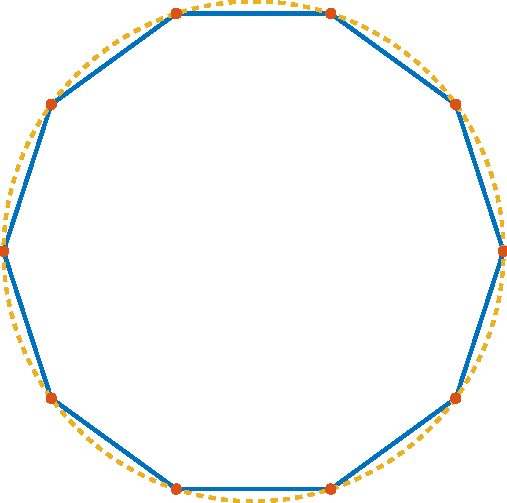
\includegraphics{Pictures/2STL.pdf}}\\
			\scalebox{0.08}{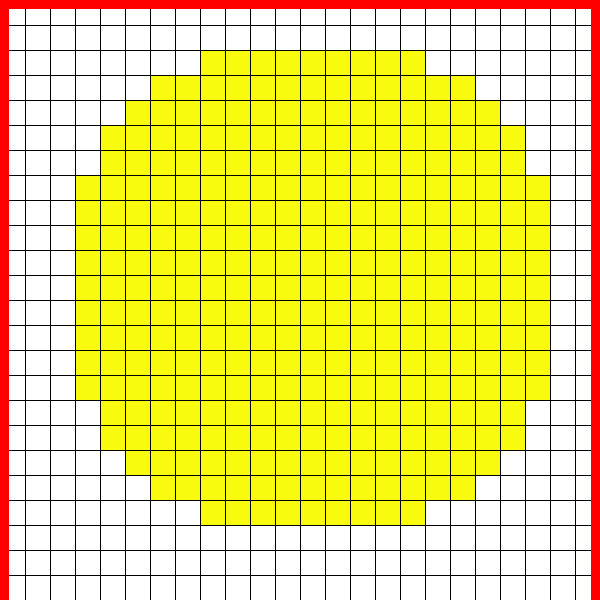
\includegraphics{Pictures/3VOXmark2.pdf}}\\
			\scalebox{0.08}{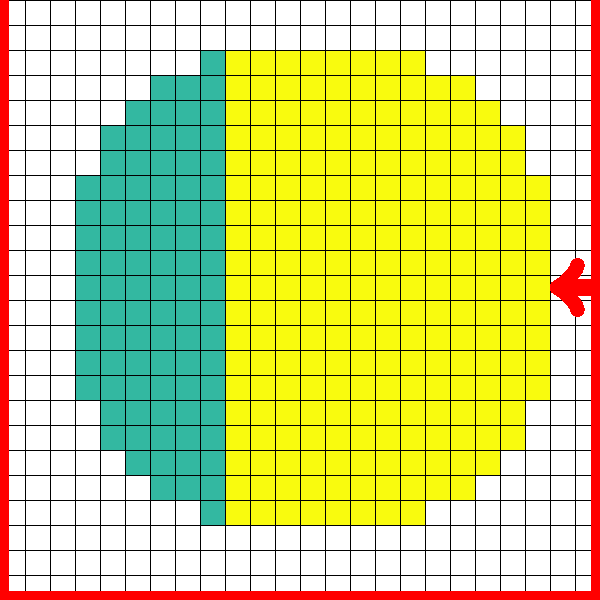
\includegraphics{Pictures/4TPDmark1.pdf}}\\
			\scalebox{0.08}{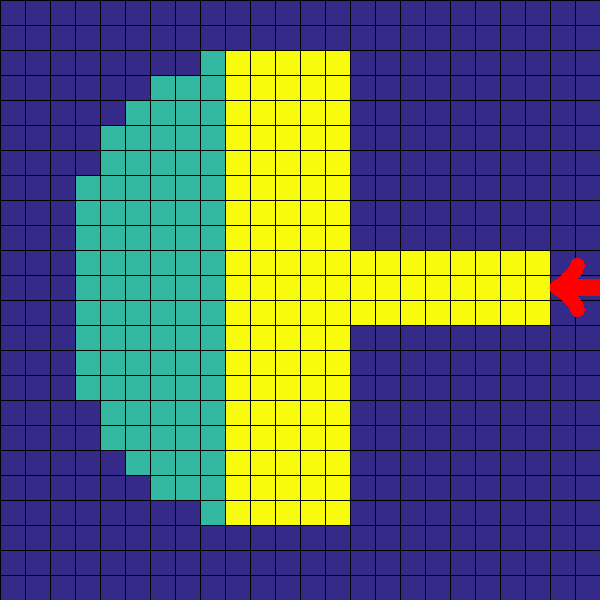
\includegraphics{Pictures/5TOPOPT.pdf}}\\
			\scalebox{0.08}{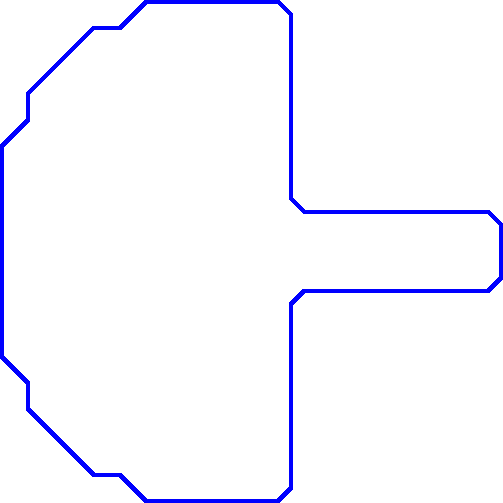
\includegraphics{Pictures/7MC.pdf}}\\
			\scalebox{0.08}{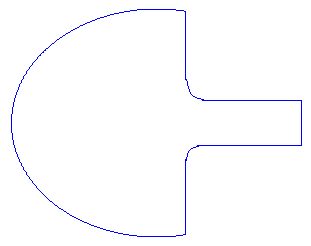
\includegraphics[scale=1.3]{Pictures/End.png}}
		\end{figure}
	\end{minipage}
\end{frame}
